\chapter{Specifica dei casi d'uso}

\section{Introduzione}
In questo documento sono analizzati ed elencati gli attori ed i casi d'uso del sistema.
Scopo del documento è la dettagliata descrizione delle modalità di interazione tra le diverse entità presenti ed il sistema.
Ciò permetterà di mettere in evidenza eventuali conflitti tra i requisiti del sistema stesso.
Tale analisi e descrizione dei casi d'uso verrà presentata tramite grafici che seguono lo standard UML.

Nei casi in cui più attori possono accedere ad un determinato caso d’uso, ma uno
solo ha come compito quella operazione, non verranno elencati tutti gli attori
ma solo quello a cui quel caso appartiene.

Inoltre non verranno riportati tutti gli attori che hanno accesso ad un dato caso d'uso ma solo quello più generico.

\section{Identificativo dei casi d'uso} %(vengono usati per definire l'ID, non ha senso metterli dopo la struttura ID)
Di seguito è spiegato come interpretare l'identificativo dei casi d'uso:
\begin{center}
	\use{categoria}{caso}%{[sottoreq]}{[\dots]}
\end{center}

\noindent
Segue una descrizione di ogni campo utilizzato nell'identificatore:
\begin{itemize}
	\item La \campiIdReq{categoria} è una lettera utilizzata per raggruppare i casi d'uso con scopi simili.
	Le categorie sono le seguenti:
	\begin{enumerateIndLabel}{\textsf{\Alph*}}{\Alph*}
		\item Autenticazione. \label{pkg:autenticazione}
		\item Gestione iscrizioni. \label{pkg:iscrizione}
		%\item Gestione iscrizioni. \label{pkg:gestioneiscrizione}
		\item Gestione vetrina. \label{pkg:vetrina} 
		\item Gestione notizie. \label{pkg:notizie}
		\item Gestione suggerimenti. \label{pkg:suggerimenti}
		\item Gestione account. \label{pkg:account}
		\item Gestione valutazioni. \label{pkg:gestionevalutazione}
		\item Gestione recensioni. \label{pkg:gestionerecensione}
		\item Interazione tra figure. \label{pkg:interazione}
		\item Gestione ticket. \label{pkg:gestioneticket}
		\item Ricerca contenuti. \label{pkg:ricerca}
		\item Gestione prodotti mancanti. \label{pkg:prodottimancanti}
		\item Visualizzazione contenuti pubblici. \label{pkg:visualizzazione}
	\end{enumerateIndLabel}

	\item Il campo \campiIdReq{caso} è un numero progressivo utilizzato per identificare in modo univoco un caso d'uso all'interno della sua categoria.
\end{itemize}

\section{Specifica degli attori}
Gli attori che interagiscono con il portale sono otto. Sono elencati e descritti di seguito:
\begin{descriptionInd}
	\item[\setTextToLabel{Visitatore}{att:visitatore}]\glsdesc*{visitatore}.

	\item[\setTextToLabel{Utente}{att:utente}]\glsdesc*{utente}.

	\item[\setTextToLabel{Produttore}{att:produttore}]\glsdesc*{produttore}.

	\item[\setTextToLabel{Redattore}{att:redattore}]\glsdesc*{redattore}.

	\item[\setTextToLabel{Assistente}{att:assistente}]\glsdesc*{assistente}.

	\item[\setTextToLabel{Moderatore}{att:moderatore}]\glsdesc*{moderatore}.

	\item[\setTextToLabel{Amministratore}{att:amministratore}]\glsdesc*{amministratore}.

	\item[\setTextToLabel{CMS}{att:cms}]\glsdesc*{cmsdef}.
\end{descriptionInd}
La gerarchia degli attori è mostrata dal seguente diagramma UML:
\begin{center}
   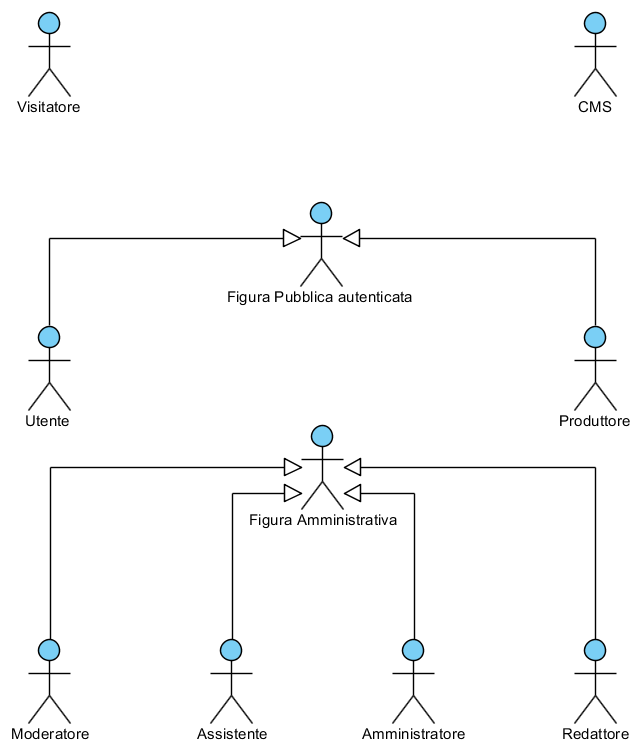
\includegraphics[width=\textwidth]{assets/visualParadigm/SchemaAttori}
\end{center}

\section{Specifica dei casi d'uso}













































%Struttura dei casi d'uso (ID) T_T
%Esempi:
%Lumiere -> Ogni caso `e identificato da una stringa del tipo CU.entit`a.sottoentit`a.caso.
%Airbnb.it -> package = PKG_<numero package>_<numero_sottopackage> | caso d'uso = UC_<numero package>_<numero caso d’uso> | attore = ATT_<num. Attore generico>_<num. Attore specifico>

%A me la struttura a package piace, possiamo racchiudere molti casi d'uso in categorie così.

%Scopiazzerei il grafico di Airbnb.it a pagina 9, utilizzando quella figura per descrivere il sistema a grandi linee, con i package. Mostrata questa, procederei con l'analisi
%dei package uno ad uno e quindi dei singoli casi d'uso.
%Per ogni caso d'uso, entrambi gli esempi fanno la descrizione stile Basi 2 con precondizioni e postcondizioni (oltre che attori coinvolti, nome, descrizione e flusso).
%A me piace


